% The Milestone 2 deck. The recorded part comes first, one frame per take in
% presentation/M2_SCRIPT.md. The appendix after the closing frame holds the
% backup slides for the interview and is never recorded.
%
% Build with `make slides-m2`, or from this folder with
% `latexmk -pdf -interaction=nonstopmode deck_m2.tex`. Asset paths are
% relative to the presentation/ directory. Every figure is drawn at the
% size of its slot by the scripts in scripts/, so its text keeps its size.
%
% The bottom-right corner of every recorded frame is kept empty for the
% webcam box, which is why the callout band is narrower than the text width.
%
% Every number that comes from a benchmark is defined once in the block
% below, from docs/RESULTS.md, so a rerun changes one place.

\documentclass[aspectratio=169,11pt]{beamer}

\usepackage[T1]{fontenc}
\usepackage{lmodern}
\usepackage{microtype}
\usepackage{xstring}
\usepackage{amsmath}
\usepackage{bm}
\usepackage{graphicx}
\usepackage{booktabs}
\usepackage{colortbl}
\usepackage{tabularx}
\usepackage{array}
\usepackage{tikz}

% ***************************************************
% Numbers, from docs/RESULTS.md
% ***************************************************

% The ladder on one node, million cell updates per second, 2048 x 512
\newcommand{\nBase}{57}
\newcommand{\nSerial}{159}
\newcommand{\nSimd}{456}
\newcommand{\nOmp}{6367}
\newcommand{\nMpiOne}{6984}
% Gain of each rung over the rung below, and total over the baseline
\newcommand{\gSerial}{2.8}
\newcommand{\gSimd}{2.9}
\newcommand{\gOmp}{14.0}
\newcommand{\xSimd}{8.0}
\newcommand{\xOmp}{112}
\newcommand{\xMpiOne}{123}
% Two nodes, 2 processes x 12 threads each, against the same layout on one node
\newcommand{\nMpiTwo}{8310}
\newcommand{\xMpiTwo}{147}
\newcommand{\twoNodeGain}{1.21}
\newcommand{\twoNodeEff}{61}
\newcommand{\twoNodeGainBig}{1.64}
\newcommand{\twoNodeEffBig}{82}
\newcommand{\exchangeShareTwo}{40}
% Strong and weak scaling
\newcommand{\strongSpeedup}{13.9}
\newcommand{\amdahlPercent}{2.4}
\newcommand{\scalarSpeedup}{18.5}
\newcommand{\weakScaled}{16}
\newcommand{\gustafsonF}{0.09}
\newcommand{\gustafsonPredicted}{22}
\newcommand{\boundaryShare}{9}
% Grid size and the roofline
\newcommand{\sizeFitsLthree}{40}
\newcommand{\gfSimd}{14}
\newcommand{\gfOmpSmall}{195}
\newcommand{\gfOmpBig}{93}
% Experiments
\newcommand{\splitGainOne}{1.19}
\newcommand{\splitGainMany}{1.12}
\newcommand{\floatGainSmall}{1.73}
\newcommand{\floatGainBig}{4.8}
\newcommand{\dynamicLoss}{43}
\newcommand{\overlapGain}{1.41}
\newcommand{\placementOneSocket}{1894}
\newcommand{\placementBothSockets}{3413}
\newcommand{\interleaveGain}{1.74}
\newcommand{\rankPerSocketGain}{2.28}

% ***************************************************
% Palette
% ***************************************************
% figstyle.py values wearing the sig* role names.

\definecolor{sigblue}{HTML}{2563EB}   % BLUE, the thing that worked
\definecolor{sigink}{HTML}{1F2937}    % titles and text
\definecolor{signavy}{HTML}{111827}   % darker ink for the head and foot bars
\definecolor{sigslate}{HTML}{6B7280}  % DARK_GREY, captions and notes
\definecolor{sigmist}{HTML}{F0F3F9}   % background canvas
\definecolor{sigcard}{HTML}{FFFFFF}   % figure and block bodies
\definecolor{sigline}{HTML}{D1D5DB}   % SPINE, hairlines
\definecolor{sigwhite}{HTML}{FFFFFF}
\definecolor{siggreen}{HTML}{059669}  % example blocks
\definecolor{sigamber}{HTML}{D97706}  % AMBER, alert blocks
\definecolor{sigred}{HTML}{DC2626}    % RED, negative results

% ***************************************************
% Theme
% ***************************************************

\usetheme{Madrid}
\usecolortheme{default}
\usefonttheme{professionalfonts}
\usefonttheme[onlymath]{serif}

\setbeamercolor{background canvas}{bg=sigmist}

\setbeamercolor*{palette primary}{bg=signavy, fg=sigwhite}
\setbeamercolor*{palette secondary}{bg=sigblue, fg=sigwhite}
\setbeamercolor*{palette tertiary}{bg=sigink, fg=sigwhite}
\setbeamercolor*{palette quaternary}{bg=signavy, fg=sigwhite}

% Every beamer element that carries a palette colour, assigned in one pass
% so the theme has a single source of truth.
\makeatletter
\@for\@entry:={%
  normal text/fg/sigink,structure/fg/sigblue,%
  itemize item/fg/sigblue,itemize subitem/fg/sigslate,%
  enumerate item/fg/sigblue,alerted text/fg/sigblue,caption name/fg/sigblue,%
  section in toc/fg/sigink,subsection in toc/fg/sigslate,%
  block title/bg/sigblue,block title/fg/sigwhite,%
  block title alerted/bg/sigamber,block title alerted/fg/sigwhite,%
  block title example/bg/siggreen,block title example/fg/sigwhite,%
  block body/bg/sigcard,block body/fg/sigink,%
  block body alerted/bg/sigcard,block body alerted/fg/sigink,%
  block body example/bg/sigcard,block body example/fg/sigink%
}\do{%
  \StrCut{\@entry}{/}\@element\@rest
  \StrCut{\@rest}{/}\@channel\@value
  % Beamer stores the key list unexpanded, so the assignment is built now.
  \edef\@assign{\noexpand\setbeamercolor{\@element}{\@channel=\@value}}%
  \@assign
}
\makeatother

\setbeamerfont{author in head/foot}{size=\tiny}
\setbeamerfont{frametitle}{size=\large}
\setbeamerfont{framesubtitle}{size=\small}
\setbeamertemplate{footline}{%
  \leavevmode%
  \hbox{%
    \begin{beamercolorbox}[wd=.44\paperwidth,ht=2.25ex,dp=1ex,center]{author in head/foot}%
      \usebeamerfont{author in head/foot}\insertshortauthor
    \end{beamercolorbox}%
    \begin{beamercolorbox}[wd=.31\paperwidth,ht=2.25ex,dp=1ex,center]{title in head/foot}%
      \usebeamerfont{title in head/foot}\insertshorttitle
    \end{beamercolorbox}%
    \begin{beamercolorbox}[wd=.25\paperwidth,ht=2.25ex,dp=1ex,right]{date in head/foot}%
      \usebeamerfont{date in head/foot}\insertshortdate{}\hspace*{2em}%
      \sigframelabel\hspace*{2ex}%
    \end{beamercolorbox}}%
  \vskip0pt%
}

\setbeamertemplate{navigation symbols}{}
\setbeamertemplate{itemize item}{\raisebox{0.15ex}{\rule{0.6ex}{0.6ex}}}
\setbeamertemplate{itemize subitem}{\raisebox{0.2ex}{\rule{0.45ex}{0.45ex}}}
\setbeamertemplate{blocks}[rounded][shadow=false]

% ***************************************************
% Slide structures
% ***************************************************

\newcommand{\sigemph}[1]{{\color{sigblue}\bfseries #1}}
\newcommand{\signote}[1]{{\color{sigslate}\footnotesize #1}}

% Row of big numbers with captions beneath. Values must not contain a slash.
\newcounter{sigentries}
\newcommand{\sigstats}[1]{%
  \setcounter{sigentries}{0}%
  \foreach \sigignored in {#1}{\stepcounter{sigentries}}%
  \pgfmathsetmacro{\sigcolwidth}{(1 - 0.04*(\value{sigentries}-1))/\value{sigentries}}%
  \par\smallskip\noindent
  \foreach \sigvalue/\sigcaption [count=\sigindex] in {#1}{%
    \ifnum\sigindex>1\hfill\fi
    \begin{minipage}[t]{\sigcolwidth\linewidth}
      \raggedright{\color{sigblue}\Large\bfseries \sigvalue}\par\vspace{0.1em}
      {\color{sigslate}\footnotesize \sigcaption}
    \end{minipage}%
  }%
  \par
}

% Tinted band across the foot of a slide for the slide's one sentence. It
% stops short of the bottom-right corner, which holds the webcam.
\newcommand{\sigcallout}[1]{%
  \vfill
  \begin{beamercolorbox}[wd=0.74\linewidth,sep=0.55em,rounded=true]{block body}
    \small{\color{sigblue}\rule{0.9ex}{0.9ex}}\hspace{0.5em}#1
  \end{beamercolorbox}%
}

% Small grey source line under the callout, for ideas not in the lectures.
\newcommand{\sigcite}[1]{\par\begin{minipage}{0.74\linewidth}\tiny\color{gray}#1\end{minipage}\par}

% Figure slot. Takes the rendered asset's path. Until the asset exists the
% slot reserves the same space and names the file it wants.
\newlength{\sigslotheight}
\setlength{\sigslotheight}{0.6\textheight}
\newcommand{\sigfigure}[2][\linewidth]{%
  \begin{minipage}{#1}
    \centering
    \IfFileExists{#2}{%
      \includegraphics[width=\linewidth,height=\sigslotheight,keepaspectratio]{#2}%
    }{%
      \setlength{\fboxsep}{0pt}%
      \fcolorbox{sigline}{sigcard}{%
        \begin{minipage}[c][\sigslotheight][c]{\dimexpr\linewidth-2\fboxrule\relax}
          \centering
          {\color{sigslate}\scriptsize\texttt{#2}}
        \end{minipage}%
      }%
    }%
  \end{minipage}%
}

% A figure on the left and plain text on the right, for diagrams and charts
% that need a line on how to read them.
\newcommand{\sigsidebyside}[3][0.57]{%
  \begin{columns}[T,onlytextwidth]
    \begin{column}{#1\textwidth}
      \sigfigure{#2}
    \end{column}
    \begin{column}{\dimexpr\textwidth-#1\textwidth-0.03\textwidth\relax}
      \small\raggedright #3
    \end{column}
  \end{columns}%
}

% Booktabs table with the rules, sizing and stretch set once.
\newcommand{\sigtable}[3]{%
  \begingroup
  \renewcommand{\arraystretch}{1.12}%
  \begin{table}\small
    \begin{tabular}{#1}
      \toprule
      #2 \\
      \midrule
      #3
      \bottomrule
    \end{tabular}
  \end{table}%
  \endgroup
}

% Appendix frames are numbered on their own, after the recorded count.
\newcounter{siglastframe}
\newif\ifsigappendix
\newcommand{\sigbackupbegin}{\setcounter{siglastframe}{\value{framenumber}}\sigappendixtrue}
\newcommand{\sigbackupend}{\setcounter{framenumber}{\value{siglastframe}}}
% The appendix divider is the first frame after the recorded ones, so the first
% backup slide is A1
\newcommand{\sigframelabel}{%
  \ifsigappendix A\the\numexpr\value{framenumber}-\value{siglastframe}-1\relax
  \else\insertframenumber{} / \inserttotalframenumber\fi}

\newcommand{\fig}[1]{../results/m2/#1}
\newcommand{\shot}[1]{../results/m2/code_shots/#1}

% ***************************************************
% Title data
% ***************************************************

\title[Parallel Heston PDE pricer]{Pricing an option on many cores}
\subtitle{SIMD, OpenMP and hybrid MPI for a Heston PDE solver}
\author[Zain Al-Saffi]{Zain Al-Saffi, 48008361}
\institute[]{COSC3500 Milestone 2}
\date{October 2026}

\begin{document}

% ==========================================================================
% The recorded part
% ==========================================================================

\begin{frame}[plain]
  \titlepage
\end{frame}

% --------------------------------------------------------------------------
\begin{frame}{The project in one slide}{Price one option by solving a PDE on a grid, then make each step parallel}
  \begin{columns}[T,onlytextwidth]
    \begin{column}{0.485\textwidth}
      \begin{block}{The question}
        What is a call option worth today, when the share price and its
        volatility both move randomly, as in the Heston model?
      \end{block}
      \begin{block}{The method}
        Solve the Heston PDE on a grid of share price by variance, stepping
        back from expiry, where every value is known, to today.
      \end{block}
    \end{column}
    \begin{column}{0.485\textwidth}
      \begin{block}{Why it parallelises}
        No cell in a step depends on another in the same step, so cells go
        to AVX2 lanes, rows to cores and blocks of rows to processes.
      \end{block}
      \begin{block}{The result}
        {\color{sigblue}\large\bfseries \xMpiOne x} on one node and
        {\color{sigblue}\large\bfseries \xMpiTwo x} on two, with the same
        answer on every version.
      \end{block}
    \end{column}
  \end{columns}
\end{frame}

% --------------------------------------------------------------------------
\begin{frame}{The problem}{The price today of the right to buy a share at a fixed price on a fixed day}
  \setlength{\sigslotheight}{0.52\textheight}
  \begin{columns}[T,onlytextwidth]
    \begin{column}{0.49\textwidth}
      \sigfigure{../results/payoff.png}
      \par\smallskip\centering\signote{At expiry the value is the payoff, max(S - K, 0).}
    \end{column}
    \begin{column}{0.49\textwidth}
      \sigfigure{\fig{f18_value_map.png}}
      \par\smallskip\centering\signote{Half way through the solve, the value above the payoff.}
    \end{column}
  \end{columns}
  \sigcallout{Black-Scholes holds the volatility constant. Heston lets the
    variance move randomly too, so the value depends on $S$, $v$ and $t$.}
\end{frame}

% --------------------------------------------------------------------------
\begin{frame}{The equation}{The value $V(S, v, t)$ solves one PDE, and each term has a plain meaning}
  \vspace*{-0.5em}
  \begin{equation*}
    V_t + \tfrac{1}{2} v S^2 V_{SS} + \rho\xi v S\, V_{Sv} + \tfrac{1}{2}\xi^2 v\, V_{vv}
    + (r - q) S\, V_S + \kappa(\theta - v)\, V_v - r V = 0
  \end{equation*}
  \vspace*{-0.6em}
  {\footnotesize
  \renewcommand{\arraystretch}{1.08}
  \begin{tabularx}{\linewidth}{@{}l X@{}}
    \toprule
    $\tfrac{1}{2} v S^2 V_{SS}$ & Diffusion in the share price, from its random movement. \\
    $\rho \xi v S V_{Sv}$ & The correlation between the share and its variance. With $\rho = -0.7$ a falling share raises volatility. \\
    $\tfrac{1}{2} \xi^2 v V_{vv}$ & Diffusion in the variance, scaled by the volatility of volatility $\xi$. \\
    $(r - q) S V_S$ & The share drifts at the risk-free rate less the dividend yield. \\
    $\kappa (\theta - v) V_v$ & Mean reversion of the variance towards its long-run level $\theta$ at rate $\kappa$. \\
    $- r V$ & Discounting, because money later is worth less than money now. \\
    \bottomrule
  \end{tabularx}}
  \sigcallout{On the grid each derivative becomes a difference of
    neighbouring cells, and one step adds $\Delta t$ times these six terms
    to the old value.}
\end{frame}

% --------------------------------------------------------------------------
\begin{frame}{One step on the grid}{From expiry $T$ to $T - \Delta t$, every new cell from nine old ones}
  \setlength{\sigslotheight}{0.62\textheight}
  \begin{center}
    \sigfigure{\fig{f13_grid.png}}
  \end{center}
  \sigcallout{A step reads only the old buffer and writes only the new one,
    so the new cells can be computed in any order.}
\end{frame}

% --------------------------------------------------------------------------
\begin{frame}{Checking the answer}{With $\xi = 0$ and $\rho = 0$ the variance never moves and Heston becomes Black-Scholes}
  \setlength{\sigslotheight}{0.62\textheight}
  \begin{center}
    \sigfigure{\fig{f14_bs_collapse.png}}
  \end{center}
  \sigcallout{With its full stencil unchanged, the solver is within 4 cents
    of the closed form at today's price. Every benchmark job runs this check
    first.}
\end{frame}

% --------------------------------------------------------------------------
\begin{frame}{The data structure}{Two flat arrays of doubles, read one, write the other, then swap}
  \setlength{\sigslotheight}{0.36\textheight}
  \begin{center}
    \sigfigure[0.9\linewidth]{\shot{shot_data_layout.png}}
  \end{center}
  \sigstats{16 KiB/one row of 2048 doubles, 8 MiB/one buffer at 2048 x 512,
    16 MiB/both buffers}
  \sigcallout{The share price axis is contiguous, so the inner loop reads
    memory in order, and a step in variance is a stride of one row.}
\end{frame}

% --------------------------------------------------------------------------
\begin{frame}{How every number was measured}{One exclusive rangpur r730 compute node, through sbatch}
  \begin{columns}[T,onlytextwidth]
    \begin{column}{0.5\textwidth}
      {\small
      \begin{itemize}
        \item Dual Xeon E5-2670 v3, 2 x 12 cores, 30 MiB L3 per socket, g++ 8.5, Open MPI 4.1.
        \item \texttt{-{}-exclusive} on a named node, so no other job shares it.
        \item Median of 5 repetitions, with the threads pinned to cores.
        \item The tests run first in the same job, and the price is printed so the compiler cannot delete the loop.
      \end{itemize}}
    \end{column}
    \begin{column}{0.46\textwidth}
      \begin{block}{A first round was discarded}
        \small Short runs leave cells below $2.2 \times 10^{-308}$, which
        this CPU handles slowly. How many there were changed with the grid,
        so the rungs ran in different regimes. Every sweep was rerun with
        those values flushed to zero.
      \end{block}
    \end{column}
  \end{columns}
  \sigcallout{Rates are million cell updates per second on the 2048 by 512
    grid unless a slide says otherwise.}
  \sigcite{Denormal numbers, D.\,Goldberg, What every computer scientist should know about floating-point arithmetic, \emph{ACM Computing Surveys} 23(1), 5 to 48, 1991.}
\end{frame}

% --------------------------------------------------------------------------
\begin{frame}{Where the time goes}{gprof flat profile, one thread, 2048 x 512}
  \setlength{\sigslotheight}{0.42\textheight}
  \begin{center}
    \sigfigure{\fig{f12_profile.png}}
  \end{center}
  \sigcallout{One function takes 99 percent of the time in every
    single-core rung, the update of the interior rows, so every rung changes
    that function.}
\end{frame}

% --------------------------------------------------------------------------
\begin{frame}{What the compiler does alone}{The baseline and serial rungs built at -O0 to -O3, the same answer at every level}
  \sigsidebyside{\fig{f11_optlevels.png}}{%
    \begin{itemize}
      \item The baseline goes from 11 at -O0 to 58 at -O2.
      \item -O3 vectorises with two-lane SSE, which doubles the baseline and gives serial 1.5x.
      \item Every benchmark builds at -O2, so each rung measures the change
        written by hand.
    \end{itemize}}
  \sigcallout{At -O3 the compiler takes the baseline to 113, still below
    the serial rung's 159 at -O2.}
\end{frame}

% --------------------------------------------------------------------------
\begin{frame}{The ladder}{Each rung adds one technique and must give the baseline's answer before it is timed}
  \sigsidebyside[0.55]{\fig{f1_ladder.png}}{%
    {\renewcommand{\arraystretch}{1.25}
    \begin{tabular}{@{}l >{\raggedright\arraybackslash}p{0.6\linewidth}@{}}
      \textbf{baseline} & the original loop, with divisions inside it \\
      \textbf{serial} & divisions turned into multiplications \\
      \textbf{simd} & four cells per AVX2 instruction \\
      \textbf{omp} & the rows shared between 24 cores \\
      \textbf{mpi} & one process per socket, edge rows exchanged \\
    \end{tabular}}}
  \sigcallout{The number inside each bar is the gain over the rung below.
    The total on one node is \sigemph{\xMpiOne x} the baseline.}
\end{frame}

% --------------------------------------------------------------------------
\begin{frame}{The serial rung}{Divisions in the loop replaced by multiplications, worked out once per solve}
  \setlength{\sigslotheight}{0.56\textheight}
  \begin{center}
    \sigfigure[0.92\linewidth]{\shot{shot_serial_change.png}}
  \end{center}
  \sigcallout{The compiler may not make this change, since the rounding can
    differ in the last bit. By hand it gives \nSerial{} million updates a second,
    \sigemph{\gSerial x}.}
\end{frame}

% --------------------------------------------------------------------------
\begin{frame}{SIMD, four cells per instruction}{Every cell in a row runs the same formula on neighbours that sit next to each other in memory}
  \sigsidebyside{\fig{f10a_simd.png}}{%
    \begin{itemize}
      \item A 256 bit AVX2 register holds four doubles.
      \item Four neighbouring cells run the same formula, so one instruction updates all four.
      \item Each group of four cells needs nine overlapping 256 bit loads.
      \item The last zero to three cells of a row are computed one at a time.
    \end{itemize}}
  \sigcallout{The serial rung already ran at 96 percent of the scalar peak,
    so the next gain came from vector instructions.}
\end{frame}

% --------------------------------------------------------------------------
\begin{frame}{SIMD code, before and after}{The serial loop and the AVX2 loop, line for line}
  \setlength{\sigslotheight}{0.62\textheight}
  \begin{center}
    \sigfigure[0.88\linewidth]{\shot{shot_simd_change.png}}
  \end{center}
  \sigcallout{Each load now reads four doubles and the update is one fused
    multiply-add, for \nSimd{} million updates a second, \sigemph{\gSimd x}
    serial.}
\end{frame}

% --------------------------------------------------------------------------
\begin{frame}{The compiler was splitting the loads}{Experiments E2 and E2b, the same source built two ways}
  \begin{columns}[T,onlytextwidth]
    \begin{column}{0.46\textwidth}
      \sigfigure{\fig{f16_split.png}}
    \end{column}
    \begin{column}{0.51\textwidth}
      \sigfigure{\shot{shot_split_loads.png}}
      \par\medskip
      {\small With only \texttt{-mavx2}, g++ 8.5 tunes for a generic x86
      and compiles every unaligned 256 bit load as two 128 bit loads.}
    \end{column}
  \end{columns}
  \sigcallout{Two flags make every unaligned load one 256 bit load, with the
    same answer and \sigemph{\splitGainOne x} the speed on one core. Every
    number in this video uses them.}
\end{frame}

% --------------------------------------------------------------------------
\begin{frame}{Could the compiler have written it?}{Experiment E1, the whole program rebuilt under stronger flags, one thread}
  \setlength{\sigslotheight}{0.58\textheight}
  \begin{center}
    \sigfigure{\fig{f15_compiler.png}}
  \end{center}
  \sigcallout{Given AVX2, g++ reaches 0.77x of the hand-written row.
    -ffast-math rewrites the divisions too, but drops the IEEE rules for
    the whole program.}
\end{frame}

% --------------------------------------------------------------------------
\begin{frame}{SIMD on the roofline}{Measured ceilings of one r730 core}
  \setlength{\sigslotheight}{0.55\textheight}
  \sigsidebyside{\fig{f5a_roofline_core.png}}{%
    \begin{itemize}
      \item The kernel does 31 flops for every 24 bytes it moves, so every rung sits on the grey vertical line.
      \item The flat lines are compute ceilings, and the sloped line is the memory bandwidth limit.
      \item The serial rung sits on the scalar peak.
    \end{itemize}}
  \sigcallout{simd does \gfSimd{} GFLOP/s, a third of the AVX2 ceiling and
    just under the one-core memory roof. On 4096 x 1024 memory slows it by
    14 percent.}
  \sigcite{S.\,Williams, A.\,Waterman and D.\,Patterson, Roofline: an insightful visual performance model for multicore architectures, \emph{Communications of the ACM} 52(4), 65 to 76, 2009.}
\end{frame}

% --------------------------------------------------------------------------
\begin{frame}{OpenMP, one block of rows per thread}{The rows of each step are shared between the cores of one node}
  \sigsidebyside{\fig{f10b_omp.png}}{%
    \begin{itemize}
      \item \texttt{schedule(static)} gives each thread one contiguous block of rows, the same block every step.
      \item Every thread reads the old buffer and writes only its own rows, so no locks are needed.
      \item The loop ends with an implicit barrier. Then the main thread updates the boundaries and swaps the buffers.
    \end{itemize}}
  \sigcallout{The code change is one pragma above the row loop.}
\end{frame}

% --------------------------------------------------------------------------
\begin{frame}{OpenMP code}{The SIMD rung's row loop, and the same loop with one pragma}
  \setlength{\sigslotheight}{0.6\textheight}
  \begin{center}
    \sigfigure[0.86\linewidth]{\shot{shot_omp_pragma.png}}
  \end{center}
  \sigcallout{On 24 cores, \nOmp{} million updates a second,
    \sigemph{\gOmp x} the SIMD rung. \texttt{default(none)} makes a
    forgotten shared variable a compile error.}
\end{frame}

% --------------------------------------------------------------------------
\begin{frame}{Strong scaling}{The same 2048 x 512 grid on 1 to 24 threads, with Amdahl's law $1/S = f + (1 - f)/p$ fitted}
  \setlength{\sigslotheight}{0.55\textheight}
  \begin{center}
    \sigfigure{\fig{f2_strong.png}}
  \end{center}
  \sigcallout{\strongSpeedup x on 24 threads, a serial fraction
    $f = \amdahlPercent$ percent. The scalar row reaches \scalarSpeedup x,
    because each of its threads needs data at a third of the rate.}
  \sigcite{Amdahl's law, COSC3500 lecture 3. Fitting $f$ to measured speedups, A.\,H. Karp and H.\,P. Flatt, Measuring parallel processor performance, \emph{Communications of the ACM} 33(5), 539 to 543, 1990.}
\end{frame}

% --------------------------------------------------------------------------
\begin{frame}{Weak scaling}{21 rows per thread, the grid grows with the threads, Gustafson's law $S = f + (1 - f)N$}
  \setlength{\sigslotheight}{0.55\textheight}
  \begin{center}
    \sigfigure{\fig{f3_weak.png}}
  \end{center}
  \sigcallout{The step time grows from 0.11 to 0.17 ms, a scaled speedup of
    \weakScaled{} on 24 threads, where Gustafson with $f = \gustafsonF$
    predicts \gustafsonPredicted.}
  \sigcite{J.\,L. Gustafson, Reevaluating Amdahl's law, \emph{Communications of the ACM} 31(5), 532 to 533, 1988.}
\end{frame}

% --------------------------------------------------------------------------
\begin{frame}{Grid size}{1 MiB to 128 MiB of working set}
  \setlength{\sigslotheight}{0.6\textheight}
  \begin{center}
    \sigfigure{\fig{f4_size.png}}
  \end{center}
  \sigcallout{While both buffers fit in the two L3 caches, 24 threads run
    \sizeFitsLthree x serial. At 4096 by 1024 they come from main
    memory and the rate halves.}
\end{frame}

% --------------------------------------------------------------------------
\begin{frame}{After threads, memory bandwidth}{Measured ceilings of the whole node}
  \setlength{\sigslotheight}{0.55\textheight}
  \sigsidebyside{\fig{f5b_roofline_node.png}}{%
    \begin{itemize}
      \item On 2048 x 512 the grid fits in the L3 caches, so the rung runs above the memory roof.
      \item On 4096 x 1024 it sits on the memory roof.
      \item The node's AVX2 ceiling of 971 GFLOP/s is five times the small grid's rate.
    \end{itemize}}
  \sigcallout{After threads the limit on the big grid is memory bandwidth,
    \gfOmpBig{} GFLOP/s at a memory roof of about 88.}
  \sigcite{S.\,Williams, A.\,Waterman and D.\,Patterson, Roofline: an insightful visual performance model for multicore architectures, \emph{Communications of the ACM} 52(4), 65 to 76, 2009.}
\end{frame}

% --------------------------------------------------------------------------
\begin{frame}{Placement}{Which socket the threads run on, and which socket's memory holds the pages}
  \setlength{\sigslotheight}{0.55\textheight}
  \begin{center}
    \sigfigure{\fig{f7_placement.png}}
  \end{center}
  \sigcallout{Two sockets give two L3 caches and two memory controllers.
    Each page is placed on the socket whose thread first writes it.}
  \sigcite{Pages and sockets, U.\,Drepper, What every programmer should know about memory, Red Hat, 2007, section 5 on NUMA.}
\end{frame}

% --------------------------------------------------------------------------
\begin{frame}{MPI, one block of rows per process}{Each process updates its own rows and receives one row from each neighbour}
  \sigsidebyside{\fig{f10c_mpi.png}}{%
    \begin{itemize}
      \item Each process owns a block of rows and keeps its own copy of the grid.
      \item To update its first and last rows it needs one row from each neighbour, held in its copied rows.
      \item So every step each process sends its edge rows and receives its neighbours'.
    \end{itemize}}
  \sigcallout{On one node, one process of 12 threads per socket fills its
    own copy of the grid, so its pages are in that socket's memory.}
\end{frame}

% --------------------------------------------------------------------------
\begin{frame}{MPI code, the time loop}{The OpenMP rung's loop, with the main changes for MPI marked}
  \setlength{\sigslotheight}{0.62\textheight}
  \begin{center}
    \sigfigure[0.88\linewidth]{\shot{shot_mpi_loop.png}}
  \end{center}
  \sigcallout{Each process updates only its own rows and the boundaries it
    owns, then exchanges its edge rows before the buffers swap.}
\end{frame}

% --------------------------------------------------------------------------
\begin{frame}{MPI code, the edge row exchange}{The receive and the send with the neighbour below, then the wait}
  \setlength{\sigslotheight}{0.6\textheight}
  \begin{center}
    \sigfigure[0.9\linewidth]{\shot{shot_mpi_exchange.png}}
  \end{center}
  \sigcallout{The receive is posted before the send, and both return
    immediately. \texttt{MPI\_Waitall} blocks until every send and receive
    has completed.}
\end{frame}

% --------------------------------------------------------------------------
\begin{frame}{Hybrid layouts}{One and two nodes, two grid sizes}
  \setlength{\sigslotheight}{0.6\textheight}
  \begin{center}
    \sigfigure{\fig{f8_layouts.png}}
  \end{center}
  \sigcallout{Two nodes give \sigemph{\twoNodeGain x} one node on the
    small grid and \sigemph{\twoNodeGainBig x} on the big one. The white
    figure is the exchange share of a step.}
\end{frame}

% --------------------------------------------------------------------------
\begin{frame}{Overlapping the exchange with the update}{Experiment E9, the edge rows sent first while the other rows are updated}
  \setlength{\sigslotheight}{0.6\textheight}
  \begin{center}
    \sigfigure{\fig{f17_overlap.png}}
  \end{center}
  \sigcallout{It helps only with one process per node, \sigemph{\overlapGain x}.
    Within a node Open MPI most likely transfers a 16 KiB row only
    during \texttt{MPI\_Waitall}.}
\end{frame}

% --------------------------------------------------------------------------
\begin{frame}{Where each step goes}{Parallel rows, serial boundaries and the edge row exchange, 2048 x 512}
  \setlength{\sigslotheight}{0.6\textheight}
  \begin{center}
    \sigfigure{\fig{f6_breakdown.png}}
  \end{center}
  \sigcallout{At 24 threads the serial boundaries take \boundaryShare{}
    percent of a step, as the main thread reads rows other cores just wrote.}
\end{frame}

% --------------------------------------------------------------------------
\begin{frame}{Same answer on every rung}{Price, delta, gamma and vega against the baseline on the test grid}
  \sigsidebyside{\fig{f9_correctness.png}}{%
    \begin{itemize}
      \item Every rung is within $3.3 \times 10^{-15}$ of the baseline, a few roundings of a double.
      \item OpenMP and MPI equal the SIMD rung bit for bit, because they split the same row updates and never sum across workers.
      \item Float, the red bar, was held to its own limit.
    \end{itemize}}
  \sigcallout{No version was timed until it matched, and every benchmark
    job reran these tests before timing anything.}
\end{frame}

% --------------------------------------------------------------------------
\begin{frame}{Tried and rejected}{Each bar is one variant against the OpenMP rung, 24 threads}
  \setlength{\sigslotheight}{0.6\textheight}
  \begin{center}
    \sigfigure{\fig{f1b_tried.png}}
  \end{center}
  \sigcallout{Dynamic scheduling lost, because every row costs the same.
    Float was faster but moved the price by 4 cents, so it was rejected.}
\end{frame}

% --------------------------------------------------------------------------
\begin{frame}{Conclusion}{The ladder against the measured ceilings}
  \vspace*{-0.4em}
  \begin{columns}[T,onlytextwidth]
    \begin{column}{0.47\textwidth}
      \sigtable{lrr}{\textbf{Rung} & \textbf{Mcell/s} & \textbf{Total}}{%
        baseline & \nBase & 1x \\
        serial & \nSerial & \gSerial x \\
        simd & \nSimd & \xSimd x \\
        omp, 24 threads & \nOmp & \xOmp x \\
        mpi, one node & \nMpiOne & \xMpiOne x \\
        \rowcolor{sigblue!12}
        mpi, two nodes & \nMpiTwo & \textbf{\xMpiTwo x} \\}
    \end{column}
    \begin{column}{0.5\textwidth}
      {\small
      \begin{itemize}
        \item Serial reached the scalar peak, so the next gain came from SIMD, and unsplit 256 bit loads added \splitGainOne x.
        \item Threads took the big grid onto the memory roof of 68 GB/s.
        \item Across nodes the exchange is the limit, and overlapping it only helps when the library sends the row immediately.
      \end{itemize}}
    \end{column}
  \end{columns}
  \sigcallout{Of the six hypotheses four held, two nodes were efficient
    only on the big grid, and the serial boundary grew with the threads.}
\end{frame}

% --------------------------------------------------------------------------
\begin{frame}{What surprised me, and what I would do next}{Looking back over the project}
  \begin{columns}[T,onlytextwidth]
    \begin{column}{0.485\textwidth}
      \begin{block}{What surprised me}
        \small
        \begin{itemize}
          \item g++ split every unaligned AVX2 load into two 128 bit loads, and the two flags that stop this made simd \splitGainOne x faster.
          \item Serial and simd ran up to 2.7x slower on a grid whose two buffers sit exactly $2^{24}$ bytes apart.
          \item Huge pages, denormals and page placement moved the rates as much as some optimisations did.
        \end{itemize}
      \end{block}
    \end{column}
    \begin{column}{0.485\textwidth}
      \begin{block}{What I would do next}
        \small
        \begin{itemize}
          \item Keep only each process's own rows in memory, so the grid can outgrow one node.
          \item Raise Open MPI's shared memory eager limit, to test why E9 only helped across nodes.
          \item Try an implicit scheme for longer timesteps, and a GPU version of the row update.
        \end{itemize}
      \end{block}
    \end{column}
  \end{columns}
  \sigcallout{Settings outside the code changed the results as much as some
    code changes, so every result file records the node, compiler and flags.}
\end{frame}

% --------------------------------------------------------------------------
\begin{frame}[plain]
  \vfill
  \centering
  {\Large\color{sigink}\bfseries \xMpiOne x on one node, \xMpiTwo x on two,
    the same answer on every rung}
  \par\vspace{0.6em}
  {\color{sigslate} Every number has a job id in docs/RESULTS.md}
  \par\vspace{0.3em}
  {\color{sigslate} COSC3500 Milestone 2, Zain Al-Saffi}
  \vfill
\end{frame}

% ==========================================================================
% The appendix. Backup slides for the interview, never recorded
% ==========================================================================

\appendix
\sigbackupbegin

\begin{frame}[plain]
  \vfill
  \centering
  {\Large\color{sigink}\bfseries Appendix}
  \par\vspace{0.6em}
  {\color{sigslate} Backup slides for questions. They are not part of the video.}
  \vfill
\end{frame}

% --------------------------------------------------------------------------
\begin{frame}{Where everything is}{The files to open, in the order the video meets them}
  {\footnotesize
  \renewcommand{\arraystretch}{1.12}
  \begin{tabularx}{\linewidth}{@{}l X@{}}
    \toprule
    \texttt{include/grid.h} & The grid, \texttt{index()} and the two buffers. \\
    \texttt{src/solver\_baseline.cpp} & Rung 0, the original loop nest with the divisions inside it. Every rung is checked against it. \\
    \texttt{src/stencil.cpp} & The constants worked out once, the scalar row and the boundaries. \\
    \texttt{src/stencil\_avx.cpp} & The AVX2 row, the only file built with \texttt{-mavx2 -mfma}, with a scalar fallback. \\
    \texttt{src/solver\_\{serial,simd,omp,mpi\}.cpp} & Rungs 1 to 4, one time loop each. \\
    \texttt{src/solver.cpp} & \texttt{make\_solver}, the stability report and reading the price off the grid. \\
    \texttt{src/solver\_experiments.cpp} & Experiments E4, E5 and E8. E2 is in \texttt{solver\_align.cpp}, E3 in \texttt{solver\_float.cpp}, E9 in \texttt{solver\_mpi.cpp}. \\
    \texttt{tests/} & Four test programs, run by \texttt{make test} and \texttt{make test-mpi}. \\
    \texttt{slurm/} & One job script per sweep, all sharing \texttt{bench\_common.sh}. \\
    \texttt{scripts/} & Every figure, drawn from the CSVs the jobs wrote. \\
    \texttt{docs/RESULTS.md} & Every number, with its job id. \\
    \bottomrule
  \end{tabularx}}
\end{frame}

% --------------------------------------------------------------------------
\begin{frame}{The Heston model}{Where the PDE comes from}
  \begin{columns}[T,onlytextwidth]
    \begin{column}{0.52\textwidth}
      \begin{block}{Two random processes}
        \vspace{-0.6em}
        \begin{align*}
          dS &= (r - q) S\,dt + \sqrt{v}\, S\, dW_S \\
          dv &= \kappa (\theta - v)\,dt + \xi \sqrt{v}\, dW_v \\
          dW_S\, dW_v &= \rho\, dt
        \end{align*}
        \vspace{-1.2em}
      \end{block}
      {\small The Feynman-Kac theorem turns the expected discounted payoff
      into the PDE. The random terms become the second derivatives, so the
      program has no random number generator.}
    \end{column}
    \begin{column}{0.44\textwidth}
      \sigtable{lr}{\textbf{Parameter} & \textbf{Value}}{%
        today's share price $S_0$ & 5200 \\
        strike $K$, expiry $T$ & 5250, 0.25 y \\
        rate $r$, dividend yield $q$ & 0.045, 0.013 \\
        $v_0 = \theta$ & 0.04 \\
        $\kappa$, $\xi$, $\rho$ & 1.5, 0.35, -0.7 \\
        grid & 2048 x 512 \\}
    \end{column}
  \end{columns}
\end{frame}

% --------------------------------------------------------------------------
\begin{frame}{The five differences}{The nine cells a step reads, and what each difference measures}
  \begin{columns}[T,onlytextwidth]
    \begin{column}{0.3\textwidth}
      \centering
      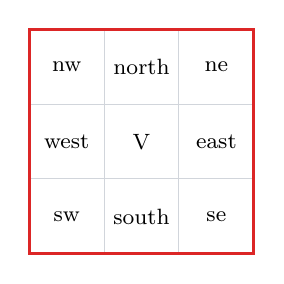
\begin{tikzpicture}[scale=0.95]
        \foreach \x/\y/\name in {0/2/nw,1/2/north,2/2/ne,0/1/west,1/1/V,2/1/east,0/0/sw,1/0/south,2/0/se}{
          \draw[fill=white, draw=sigline] (\x,\y) rectangle ++(1,1);
          \node[font=\footnotesize] at (\x+0.5,\y+0.5) {\name};
        }
        \draw[very thick, sigred] (0,0) rectangle (3,3);
      \end{tikzpicture}
      \par\smallskip\signote{share price across, variance up}
    \end{column}
    \begin{column}{0.68\textwidth}
      {\footnotesize
      \renewcommand{\arraystretch}{1.2}
      \begin{tabular}{@{}l l >{\raggedright\arraybackslash}p{0.42\linewidth}@{}}
        \toprule
        & \textbf{difference} & \textbf{what it measures} \\
        \midrule
        $V_S$ & (east $-$ west) $/\, 2\Delta S$ & how steeply value rises with share price \\
        $V_{SS}$ & (east $- 2V +$ west) $/\, \Delta S^2$ & how curved it is along the share price \\
        $V_v$ & (north $-$ south) $/\, 2\Delta v$ & how value changes with variance \\
        $V_{vv}$ & (north $- 2V +$ south) $/\, \Delta v^2$ & how curved it is along the variance \\
        $V_{Sv}$ & (ne $-$ nw $-$ se $+$ sw) $/\, 4\Delta S \Delta v$ & how the share slope changes with variance, which is why the corners are needed \\
        \bottomrule
      \end{tabular}}
    \end{column}
  \end{columns}
  \par\medskip
  {\small The serial rung multiplies by $1/(2\Delta S)$ and the others,
  worked out once per solve, where the baseline divides in every cell.}
\end{frame}

% --------------------------------------------------------------------------
\begin{frame}{The boundaries}{Each edge of the grid has its own rule, all serial in the OpenMP rung}
  {\small
  \renewcommand{\arraystretch}{1.25}
  \begin{tabularx}{\linewidth}{@{}l X@{}}
    \toprule
    $v = 0$, the bottom row & Every diffusion term has a factor $v$, so only the drift terms are left. $V_v$ looks one row up, because there is no row below. \\
    $S = 0$, the first column & A call is worth nothing there. A put is worth the discounted strike. \\
    largest $S$, the last column & A call is worth $S e^{-q\tau} - K e^{-r\tau}$ there, and a put nothing. \\
    the top variance row & A copy of the row below, so the value stops changing with variance at the top. It runs last. \\
    \bottomrule
  \end{tabularx}}
  \sigcallout{On one thread the boundaries are 0.4 percent of a step. At 24
    threads they are \boundaryShare{} percent, because the main thread has
    to fetch rows that other cores just wrote.}
\end{frame}

% --------------------------------------------------------------------------
\begin{frame}{The timestep limit}{An explicit scheme is only stable below a largest timestep}
  \begin{equation*}
    \Delta t_{\text{stable}} = \frac{1}{v_{\max} S_{\max}^2 / \Delta S^2 + \xi^2 v_{\max} / \Delta v^2 + r}
  \end{equation*}
  {\small
  \begin{itemize}
    \item The far corner of the grid is the worst cell, where the diffusion is largest.
    \item At 2048 x 512 the limit is $3.66 \times 10^{-7}$ years, so the real three-month solve takes 980000 steps.
    \item Every benchmark picks its maturity so that $\Delta t$ is 70 percent of the limit (\texttt{maturity\_for} in \texttt{bench\_common.sh}).
    \item Above the limit the solution grows without bound and the price comes out as \texttt{nan}.
  \end{itemize}}
\end{frame}

% --------------------------------------------------------------------------
\begin{frame}{Why an explicit scheme}{Each new cell comes straight from known values}
  {\small
  \begin{itemize}
    \item An explicit step computes each new cell from the old buffer, $V^{\text{new}} = V + \Delta t \times$ (the six terms), with no equation to solve.
    \item So the work is a stencil, regular and local, which splits cleanly between lanes, threads and processes.
    \item An implicit scheme would solve a linear system across the whole grid every step, which couples the cells and is much harder to parallelise.
    \item The cost of the explicit choice is the timestep limit, so the solver takes many small steps. Each step is the same regular work, which suits SIMD, threads and processes.
  \end{itemize}}
\end{frame}

% --------------------------------------------------------------------------
\begin{frame}{Reading the price and the Greeks}{\texttt{extract\_result} in \texttt{src/solver.cpp}, after the last step}
  {\small
  \begin{itemize}
    \item Today's share price and variance fall between grid nodes, so the price is interpolated bilinearly from the four cells around that point.
    \item The same interpolation one cell to each side gives the values the Greeks need.
    \item Delta and gamma are central differences in the share price, and vega a central difference in the variance, per unit of variance.
    \item The solver says on stderr when the quote is off a node, so an interpolated price is never mistaken for a node value.
  \end{itemize}}
\end{frame}

% --------------------------------------------------------------------------
\begin{frame}{Flops and bytes per cell}{Where the roofline's x position comes from}
  \begin{columns}[T,onlytextwidth]
    \begin{column}{0.5\textwidth}
      \begin{block}{31 flops per cell update}
        \small 15 for the five differences and 16 to add up the PDE terms
        and step. A fused multiply-add counts as two.
      \end{block}
    \end{column}
    \begin{column}{0.46\textwidth}
      \begin{block}{24 bytes per cell update}
        \small 8 to read the old value, 8 to write the new one, and 8 more
        because a store first reads the cache line it writes into.
      \end{block}
    \end{column}
  \end{columns}
  \par\medskip
  {\small The arithmetic intensity is $31/24 = 1.29$ flops per byte. The
  rate in GFLOP/s is the measured cell updates per second times 31. The
  ceilings come from \texttt{slurm/bench\_peak.sh} on the same node, a
  scalar and an AVX2 FMA loop for compute and a triad for memory.}
\end{frame}

% --------------------------------------------------------------------------
\begin{frame}{The AVX2 row next to the scalar row}{The same sum, one cell or four}
  \setlength{\sigslotheight}{0.74\textheight}
  \begin{center}
    \sigfigure[0.8\linewidth]{\shot{shot_simd_fma.png}}
  \end{center}
\end{frame}

% --------------------------------------------------------------------------
\begin{frame}{Why SIMD is below 4x}{Four lanes, \gSimd x measured}
  {\small
  \begin{itemize}
    \item Each group of four cells needs nine overlapping 4-wide loads, plus two for the $S$ and $S^2$ tables.
    \item The west, centre and east loads are 8 bytes apart, so at most one of them can start on a 32 byte boundary. Every unaligned load crosses a cache line on every other iteration, which moves the rate by up to 16 percent (E2b).
    \item At \nSimd{} million updates a second one core moves about 11 GB/s, close to the 12.4 GB/s it can stream from memory.
    \item The last zero to three cells of every row are computed one at a time, and each row first loads its constants into registers.
  \end{itemize}}
  \sigcallout{No hardware counters were available in the jobs, so the loss
    cannot be split exactly between these causes.}
\end{frame}

% --------------------------------------------------------------------------
\begin{frame}{Where the rows sit in their cache lines}{Experiment E2b, one thread, 2048 x 512, with unsplit loads}
  \sigtable{lr}{\textbf{Where column 1 sits} & \textbf{Mcell/s}}{%
    centre load on a 32 byte boundary & 477 \\
    west or east load on a 32 byte boundary & 439 \\
    no load on a 32 byte boundary & 412 \\
    aligned load instructions, centre aligned & 477 \\
    east and west built by register shuffles & 460 \\}
  {\small An aligned load instruction runs at the same speed as an unaligned
  one at the same address. The rate depends on whether a load crosses a
  cache line.}
\end{frame}

% --------------------------------------------------------------------------
\begin{frame}{Experiment E1 in full}{The whole program rebuilt under each set of flags, one thread, 2048 x 512, Mcell/s}
  {\footnotesize
  \renewcommand{\arraystretch}{1.05}
  \begin{tabularx}{\linewidth}{@{}X rrr@{}}
    \toprule
    \textbf{Build} & \textbf{baseline} & \textbf{serial} & \textbf{simd} \\
    \midrule
    \texttt{-O2}, shipped & 57.6 & 157.0 & 449.6 \\
    \texttt{-O3} & 112.5 & 241.3 & 446.9 \\
    \texttt{-O3 -mavx2 -mfma} & 107.4 & 345.6 & 451.1 \\
    \texttt{-O3 -mavx2 -mfma}, unsplit loads in the whole program & 106.4 & 362.7 & 452.0 \\
    \texttt{-O3 -march=native} & 105.9 & 266.3 & 455.8 \\
    \texttt{-O2 -ffast-math} & 58.6 & 175.1 & 476.5 \\
    \texttt{-O3 -ffast-math} & 189.5 & 271.5 & 472.7 \\
    \texttt{-O3 -mavx2 -mfma -ffast-math} & 380.1 & 468.2 & 478.0 \\
    \texttt{-O3 -mavx2 -mfma -ffast-math}, unsplit loads in the whole program & 376.8 & 399.3 & 478.2 \\
    \bottomrule
  \end{tabularx}}
  \par\smallskip
  {\footnotesize The simd column always has unsplit loads, from the two flags
  on its own file. Every build gives the \texttt{-O2} answers to within
  $1.1 \times 10^{-14}$. Why \texttt{-march=native} slows serial, and why
  the fast-math serial rung is slower with unsplit loads, has not been found.
  Jobs 659248 and 659249.}
\end{frame}

% --------------------------------------------------------------------------
\begin{frame}{Why there are no locks}{\texttt{schedule(static)}, \texttt{default(none)} and the barrier}
  {\small
  \begin{itemize}
    \item Each thread reads only \texttt{current} and writes only its own rows of \texttt{next}. No cell is written by two threads, and no thread reads \texttt{next} during the loop.
    \item \texttt{schedule(static)} splits the rows into equal contiguous blocks once. Every row costs the same, so dynamic scheduling only added overhead (E5, up to \dynamicLoss{} percent slower).
    \item \texttt{default(none)} makes every variable used in the loop be listed. The loop counter and the variables inside the body are private to each thread.
    \item The parallel loop ends with an implied barrier, so every row is done before the boundaries and the swap.
  \end{itemize}}
\end{frame}

% --------------------------------------------------------------------------
\begin{frame}{The swap}{Two references bound once, still right after every swap}
  \setlength{\sigslotheight}{0.5\textheight}
  \begin{center}
    \sigfigure[0.8\linewidth]{\shot{shot_swap.png}}
  \end{center}
  {\small \texttt{std::swap} on two vectors swaps their internal pointers
  and copies no numbers. The references name the two member vectors, so
  after the swap \texttt{current} holds what was just written.}
\end{frame}

% --------------------------------------------------------------------------
\begin{frame}{Constants copied into local variables}{Why the row starts with a block of copies}
  \setlength{\sigslotheight}{0.5\textheight}
  \begin{center}
    \sigfigure[0.86\linewidth]{\shot{shot_locals.png}}
  \end{center}
  {\small The row writes through a \texttt{double*}, and the compiler cannot
  prove that pointer never points into the constants. Without the copies it
  would reload every constant after every store. As locals they stay in
  registers for the whole row.}
\end{frame}

% --------------------------------------------------------------------------
\begin{frame}{Amdahl and Gustafson}{The two laws with the measured numbers}
  \begin{columns}[T,onlytextwidth]
    \begin{column}{0.48\textwidth}
      \begin{block}{Amdahl, a fixed problem}
        \small $S(p) = 1 / \big(f + (1 - f)/p\big)$. Fitted by least
        squares to the strong scaling speedups, $f = \amdahlPercent$ percent,
        more than five times the 0.44 percent of boundary work on one
        thread. The rest is the fork and barrier every step and the shared
        cache bandwidth. The scalar row fits 1.6 percent, because a faster
        row makes those fixed costs a larger share of each step.
      \end{block}
    \end{column}
    \begin{column}{0.48\textwidth}
      \begin{block}{Gustafson, a growing problem}
        \small $S(N) = f + (1 - f) N$, with $f$ the serial share of the
        parallel run. Measured on 24 threads $f = \gustafsonF$, which
        predicts \gustafsonPredicted. The measured scaled speedup is
        \weakScaled.
      \end{block}
    \end{column}
  \end{columns}
  \sigcite{Karp and Flatt 1990, Gustafson 1988, as on the scaling slides.}
\end{frame}

% --------------------------------------------------------------------------
\begin{frame}{Thread binding on the r730 nodes}{Why \texttt{close} alternates sockets}
  {\small
  \begin{itemize}
    \item The CPUs are numbered even on socket 0 and odd on socket 1 (job 651500 printed each thread's CPU).
    \item \texttt{OMP\_PLACES=cores OMP\_PROC\_BIND=close} fills CPUs 0, 1, 2, so every even thread count is split evenly over the two sockets.
    \item \texttt{spread} with fewer than 24 threads stays on socket 0, which is how E6 measured one socket against two.
    \item Unbound threads were 1.11x faster on the small grid at 24 threads, which is not explained. On the big grid the reps range from 2699 to 4009 within one job, so the comparison there is noise.
  \end{itemize}}
\end{frame}

% --------------------------------------------------------------------------
\begin{frame}{Page placement, numactl and huge pages}{Where the memory of the grid comes from}
  {\small
  \begin{itemize}
    \item Linux places a page in the memory of the socket whose thread first writes it, which is called the first-touch policy. The grid is filled by the main thread, so every page is on socket 0.
    \item \texttt{numactl -{}-interleave=all} spreads the pages over both sockets, \interleaveGain x on the big grid (E7). Without it the runs fall into two groups, near 2800 and near 4000, so the size of the gain depends on which group they fall in.
    \item One MPI process per socket allocates and fills its own copy, so its pages are local, \rankPerSocketGain x on the big grid.
    \item \texttt{MALLOC\_MMAP\_THRESHOLD\_=1048576} makes every buffer over 1 MiB come from \texttt{mmap}, so each repetition gets fresh 2 MiB huge pages. Without it only the first repetition gets them (E11, 0.63x on 24 threads).
  \end{itemize}}
  \sigcite{U.\,Drepper, What every programmer should know about memory, Red Hat, 2007, section 5.}
\end{frame}

% --------------------------------------------------------------------------
\begin{frame}{Which rows a process owns}{\texttt{rows\_for\_rank}, and \texttt{MPI\_Gatherv} at the end}
  \setlength{\sigslotheight}{0.56\textheight}
  \begin{center}
    \sigfigure[0.8\linewidth]{\shot{shot_rows_for_rank.png}}
  \end{center}
  {\small When the rows do not divide evenly the first processes take one
  more row each. At the end \texttt{MPI\_Gatherv} collects the blocks, with
  one count and offset per process, outside the timed steps.}
\end{frame}

% --------------------------------------------------------------------------
\begin{frame}{E9 in code}{The edge rows first, then the messages, then the other rows}
  \setlength{\sigslotheight}{0.6\textheight}
  \begin{center}
    \sigfigure[0.86\linewidth]{\shot{shot_overlap.png}}
  \end{center}
  {\small \texttt{barrier} makes every thread finish the rows the
  neighbours need. \texttt{master} lets one thread post the messages, and
  unlike \texttt{single} it has no barrier at its end.}
\end{frame}

% --------------------------------------------------------------------------
\begin{frame}{Why E9 only helped across nodes}{How Open MPI 4.1.1 moves a message, read from \texttt{ompi\_info} on rangpur}
  {\small
  \begin{itemize}
    \item Between nodes it uses TCP, whose eager limit is 64 KiB, so a 16 KiB row is sent as soon as \texttt{MPI\_Isend} is called.
    \item Between processes on one node it uses shared memory, whose eager limit is 4 KiB. A 16 KiB row uses the rendezvous protocol and is only transferred once the receiver is inside an MPI call.
    \item There is no progress thread, so that call is \texttt{MPI\_Waitall} at the end of the step, and the transfer does not overlap the update.
    \item The only layout that gained, one process on each of two nodes, is the only one with no two processes on one node.
  \end{itemize}}
  \sigcallout{This explanation fits every small grid layout but has not been
    tested. Raising the shared memory eager limit above 16 KiB would test it.}
\end{frame}

% --------------------------------------------------------------------------
\begin{frame}{The two node numbers between jobs}{The same build and layouts, run minutes apart, Mcell/s}
  \sigtable{lrrrr}{\textbf{Layout} & \textbf{2048, job 659242} & \textbf{job 659243} & \textbf{4096, job 659242} & \textbf{job 659243}}{%
    1 node, 1 x 24 & 6233 & 6288 & 2907 & 3045 \\
    1 node, 2 x 12 & 6843 & 7025 & 6624 & 6664 \\
    2 nodes, 1 x 24 & 7064 & 5693 & 9002 & 9262 \\
    2 nodes, 2 x 12 & 8310 & 9364 & 10863 & 10848 \\}
  {\small The two node layouts on the small grid differ between the jobs by
  more than the repetitions inside one job do. Every other layout agrees
  within 5 percent. So the two node gain on the small grid lies between
  \twoNodeGain x and 1.33x.}
  \sigcallout{The headline quotes job 659242, which the hybrid figure is
    drawn from. Job 659243 is the E9 job, and these are its \texttt{mpi} rows.}
\end{frame}

% --------------------------------------------------------------------------
\begin{frame}{MPI started for threads}{\texttt{MPI\_Init\_thread} with \texttt{MPI\_THREAD\_FUNNELED}}
  \setlength{\sigslotheight}{0.4\textheight}
  \begin{center}
    \sigfigure[0.86\linewidth]{\shot{shot_init_thread.png}}
  \end{center}
  {\small FUNNELED tells MPI that only the main thread calls it while
  OpenMP threads run. The \texttt{mpi} rung calls MPI only outside parallel
  regions. The \texttt{mpi\_overlap} rung calls it from the master thread
  inside one, so it checks the level and refuses to run below it.}
\end{frame}

% --------------------------------------------------------------------------
\begin{frame}{The test that timed out}{One 3-process solve of the test grid under three settings}
  \sigtable{lrrr}{\textbf{Solver} & \textbf{close, on cores} & \textbf{passive wait} & \textbf{not bound}}{%
    simd & 1.05 s & 1.04 s & 0.62 s \\
    omp & 1.04 s & 1.12 s & 0.59 s \\
    mpi & 14.24 s & 1.16 s & 0.58 s \\
    mpi\_overlap & 14.66 s & 1.17 s & 0.60 s \\}
  {\small The bench scripts pinned threads to cores, and the MPI test
  inherited that, so every process put its two threads on cores 0 and 1.
  Waiting OpenMP threads busy-wait, so one process held the cores its neighbour needed
  to finish and send its row. The test now sets
  \texttt{OMP\_PROC\_BIND=false}, and validation fell from 14 to 2.5
  minutes.}
\end{frame}

% --------------------------------------------------------------------------
\begin{frame}{Denormal numbers}{Flushed to zero by a library loaded before \texttt{main}}
  \begin{columns}[T,onlytextwidth]
    \begin{column}{0.55\textwidth}
      \sigfigure{\shot{shot_flush_denormals.png}}
      \par\smallskip
      {\footnotesize \texttt{\_\_attribute\_\_((constructor))} runs the
      function before \texttt{main}. It sets flush to zero and denormals are
      zero in the SSE control register. The bench scripts load it with
      \texttt{LD\_PRELOAD}, so \texttt{heston} itself is unchanged.}
    \end{column}
    \begin{column}{0.42\textwidth}
      \sigtable{lrr}{\textbf{Rung} & \textbf{as is} & \textbf{flushed}}{%
        baseline & 53 & 57 \\
        serial & 124 & 159 \\
        simd & 320 & 454 \\
        omp 24 & 4865 & 6484 \\}
      {\footnotesize Job 659436. Every price is identical to ten digits
      either way.}
    \end{column}
  \end{columns}
\end{frame}

% --------------------------------------------------------------------------
\begin{frame}{The 2\textsuperscript{24} byte address effect}{A slow point in the grid size sweep, caused by where the two buffers sit in memory}
  {\small
  \begin{itemize}
    \item With split loads, simd on one thread ran at 169 to 183 on any grid whose two buffers sit exactly $2^{24}$ bytes apart, such as 2896 x 724, 1448 x 1448 and 2044 x 1026, and about 405 on the grids next to them. With unsplit loads it still runs at 169 at 2896 x 724.
    \item omp on 2 threads shows the same, 336 against 814. Serial is slow there too on the current code, 58 at 2896 x 724.
    \item omp on 24 threads ran at 6499 there in two earlier jobs, and at 3288 and 3267 in the latest two, one with each build, so the flags are not the cause.
    \item The grids that trigger it are known, and the hardware mechanism has not been found.
  \end{itemize}}
  \sigcallout{That is why the 2896 x 724 points are hollow on the grid size
    figure, and why its 56x is left out.}
\end{frame}

% --------------------------------------------------------------------------
\begin{frame}{Float instead of double}{Experiment E3, faster and still rejected}
  {\small
  \begin{itemize}
    \item Float halves the bytes per cell and doubles the lanes per register. On one thread 1.92x simd, on 24 threads \floatGainSmall x on 2048 x 512 and \floatGainBig x on 4096 x 1024.
    \item The big grid gains most, because the float buffers (32 MB) fit in the two L3 caches (60 MB) and the double buffers (64 MB) do not.
    \item On the reference solve the float price is 196.1256 against 196.1684 in double and 196.1692 from Fourier inversion. The 4 cent error is larger than the discretisation error of a much coarser double grid.
    \item Gamma moved by 11.9 percent, vega by 2.3 and delta by 0.46.
  \end{itemize}}
\end{frame}

% --------------------------------------------------------------------------
\begin{frame}{The six hypotheses}{Written before the sweeps ran, then checked against them}
  \sigtable{c >{\raggedright\arraybackslash}p{0.42\linewidth} >{\raggedright\arraybackslash}p{0.4\linewidth}}{\textbf{\#} & \textbf{Hypothesis} & \textbf{Outcome}}{%
    1 & SIMD gives 2 to 3.5x over serial & held, \gSimd x \\
    2 & OpenMP scales close to linearly to 12 threads & mostly held, 9.6x on 12 threads, 80 percent efficient \\
    3 & the large grid becomes memory-bound & held, on the memory roof at 4096 x 1024 \\
    4 & the serial boundary stays near 0.5 percent & overturned, \boundaryShare{} percent at 24 threads \\
    5 & one process per socket beats one of 24 threads & held, 1.10x and \rankPerSocketGain x \\
    6 & two nodes above 80 percent efficient & overturned at 2048 x 512, \twoNodeEff{} percent. Held at 4096 x 1024, \twoNodeEffBig{} percent \\}
\end{frame}

% --------------------------------------------------------------------------
\begin{frame}{What the tests check}{Run by \texttt{make test} and \texttt{make test-mpi} before every benchmark}
  {\small
  \renewcommand{\arraystretch}{1.2}
  \begin{tabularx}{\linewidth}{@{}l X@{}}
    \toprule
    \texttt{test\_bs\_collapse} & With $\xi = 0$ and $v_0 = \theta$ the variance never moves, and the solver must match Black-Scholes. \\
    \texttt{test\_parity} & Put-call parity, $C - P = S e^{-qT} - K e^{-rT}$, on the full model. It holds in any model, so a gap means a bug. \\
    \texttt{test\_ladder\_matches} & Every rung against the baseline within $10^{-11}$, and the parallel rungs against simd to the bit, at 1, 2 and 7 threads and on 2 and 3 processes. \\
    \texttt{test\_avx\_row} & The AVX2 row against the scalar row on random grid values. \\
    \bottomrule
  \end{tabularx}}
  \sigcallout{7 threads and 3 processes do not divide the 32 test rows
    evenly, so the uneven split is tested too.}
\end{frame}

% --------------------------------------------------------------------------
\begin{frame}{How the figures were made}{Every figure is drawn by a script from files the jobs wrote}
  {\footnotesize
  \renewcommand{\arraystretch}{1.15}
  \begin{tabularx}{\linewidth}{@{}l X@{}}
    \toprule
    \texttt{scripts/m2\_figures.py} & Every benchmark chart, from the sweep CSVs, the peak file, a test log and the gprof output. Each bar or point is the median of 5 repetitions in one exclusive job. \\
    \texttt{scripts/decomposition\_diagram.py} & The three diagrams of who owns which cells. \\
    \texttt{scripts/method\_figures.py} & The grid step, the Black-Scholes check and the value map, the last two from \texttt{heston -{}-dump-every} snapshots. \\
    \texttt{scripts/payoff\_diagram.py} & The payoff. \\
    \texttt{scripts/code\_shots.py} & The code images, from the source files, with the file and lines on each. \\
    \bottomrule
  \end{tabularx}}
  \sigcallout{\texttt{make m2-figures} and \texttt{make code-shots} redraw
    everything. The script refuses any CSV whose host is not a compute
    node.}
\end{frame}

% --------------------------------------------------------------------------
\begin{frame}{Tests before timing}{The job stops unless every test passes}
  \setlength{\sigslotheight}{0.5\textheight}
  \begin{center}
    \sigfigure[0.9\linewidth]{\shot{shot_iron_rule.png}}
  \end{center}
  {\small Every benchmark job builds from clean, runs \texttt{make test},
  \texttt{make test-mpi} and \texttt{make avx-check}, and only then times
  anything.}
\end{frame}

% --------------------------------------------------------------------------
\begin{frame}{Where a number came from}{The header every benchmark CSV carries, written by the job}
  \setlength{\sigslotheight}{0.74\textheight}
  \begin{center}
    \sigfigure[0.96\linewidth]{\shot{shot_csv_header.png}}
  \end{center}
\end{frame}

\sigbackupend
\end{document}
